\section{Silizium-PVD}
\label{siliconpvd}

Mit Silizium soll ein weiteres PVD-Material untersucht werden, das im Gegensatz zu den bisher untersuchten Metallen, welche ungerichtete Bindungen aufbauen und damit die kristalline Strukturen bevorzugen, auf gerichteten Bindungen beruht.
Deshalb werden reaktive Kraftfelder genutzt, welche auf einer expliziten Beschreibung gerichteter Bindungen über Bindungsordnungen benachbarter Atome basieren.

\subsection{Verfügbare ReaxFF-Parametrisierungen}

Da die ReaxFF-Formulierung erst innerhalb des letzten Jahrzehntes an Popularität gewonnen hat, sind die verfügbaren Potentiale auf sehr spezielle Probleme angepasst und unterstützen meist entweder Bulkmaterialien oder Reaktionen zwischen Molekülen.
Tabelle~\ref{tab:siliconpotentials} listet die im Rahmen der Arbeit untersuchten ReaxFF-Parametrisierungen auf, die in der Literatur gefunden werden konnten.

\begin{table}[hb]
  \caption{Untersuchte ReaxFF-Parametrisierungen für Silizium- und Siliziumoxidsysteme}
  \label{tab:siliconpotentials}
  \oddrowcolors
  \begin{tabularx}{1\textwidth}{|lXc|}
    \hline
    \textbf{Bezeichnung}  & \textbf{Anwendung \& Kommentare}                                                                          & \textbf{Ref.}                     \\
    \hline
    \pot{Al\_Al0\_AlN}    & \ce{Al}, \ce{Al2O3}, \ce{AlN}. Basiert auf einer Si-Parametrisierung                                      & \cite{plimpton_lammps_2014}       \\
    \pot{chenoweth}       & Zersetzung von Polydimethylsiloxane bei hohen Drücken und Temperaturen. Ergänzung von \ce{C-Si}-Bindungen & \cite{chenoweth_simulations_2005} \\
    \pot{kulkarni}        & Reaktion von Sauerstoff mit \ce{OH}-terminierten Siliziumoxid-Oberflächen                                 & \cite{kulkarni_oxygen_2013}       \\
    \pot{lg}              & ``low gradients''. Siehe liu\_nitramines. Fehlerhafte Version aus LAMMPS                                  & \cite{liu_reaxff-lg:_2011}        \\
    \pot{liu\_ettringite} & Verspannung von Ettringit (\ce{Ca6[Al(OH)6]2(SO4)3 26H2O}). Basiert auf Si-Parametrisierung               & \cite{liu_development_2012}       \\
    \pot{liu\_nitramines} & Dichtebestimmung von Nitramin-Molekülen bei hohen Drücken. Dichte erhöht durch Van-der-Waals-Korrekturen  & \cite{liu_reaxff-lg:_2011}        \\
    \pot{narayanan}       & Präparation mit \ce{Li-Al}-Silikaten. Für Phasenübergänge von Eukryptit-Kristallen (\ce{LiAl[SiO4]})      & \cite{narayanan_reactive_2012}    \\
    \pot{newsome}         & Oxidation von \ce{SiC}-Oberflächen mit \ce{O2} und \ce{H2O} bei \SIrange{500}{5000}{\kelvin}              & \cite{newsome_oxidation_2012}     \\
    \pot{nielson}         & Reaktionskinetik an Metallkatalysatoren bei hohen Temperaturen                                            & \cite{nielson_development_2005}   \\
    \pot{zhang}           & Zersetzung energetischer Moleküle (Nitramin-Explosionen)                                                  & \cite{zhang_carbon_2009}          \\
    \hline
  \end{tabularx}
\end{table}

\subsection{Voruntersuchungen}

In Ergänzung zu den bisherigen Voruntersuchungen, welche sich entsprechend der erwarteten Strukturen der abgeschiedenen Schichten auf die Beschreibung kristalliner Strukturen beschränkten, werden für die Silizium-Parametrisierungen auch die Eigenschaften amorpher Strukturen untersucht.
Die verwendeten Methoden wurden bereits in Abschnitt~\ref{mdmethods} vorgestellt.
Diese zusätzlichen Untersuchungen haben umfassendere Aussagen über die Anwendbarkeit der Parametrisierungen für vollständige Abscheidungssimulationen zum Ziel.
Die Ergebnisse dieser Betrachtungen sind in Tabelle~\ref{tab:siliconpreresults} zusammen gefasst und werden im Weiteren kurz diskutiert.

\begin{table}[th]
  \begin{threeparttable}
    \caption[Zusammenfassung der Voruntersuchungen für Silizium-Systeme]{
      Zusammenfassung der Voruntersuchungen für Silizium-Systeme.
      Siehe Anhang~\ref{appendix_silicon}
    }
    \label{tab:siliconpreresults}

    \oddrowcolors
    \begin{tabularx}{\textwidth}{|lCCCCCCC|}
      \hline
      \textbf{Bezeichnung}    & LMP\tnote{a} & c-\ce{Si} & c-\ce{SiO2} & a-\ce{Si} & \ce{SiH4} & \ce{+O2} & PVD\tnote{b} \\
      \hline                % & LAMMPS       & c-Si      & c-SiO2      & a-Si      & Silane    & +O2      & PVD          \\
      \pot{Al\_Al0\_AlN}      & \cmark       & ~         & (\cmark)    & \cmark    & \cmark    & ~        & \cmark       \\
      \pot{chenoweth}         & ~            & ~         & ~           & ~         & ~         & ~        & ~            \\
      \pot{kulkarni}          & \cmark       & \cmark    & \cmark      & \cmark    & \cmark    & (\cmark) & \cmark       \\
      \pot{lg}                & ~            & ~         & ~           & ~         & ~         & ~        & ~            \\
      \pot{liu\_ettringite}   & \cmark       & ~         & \cmark      & \cmark    & ~         & ~        & \cmark       \\
      \pot{liu\_nitramines}   & ~            & ~         & ~           & ~         & ~         & ~        & ~            \\
      \pot{narayanan}         & \cmark       & ~         & \cmark      & \cmark    & ~         & ~        & \cmark       \\
      \pot{newsome}           & \cmark       & ~         & (\cmark)    & ~         & ~         & (\cmark) & \cmark       \\
      \pot{nielson}           & \cmark       & \cmark    & \cmark      & \cmark    & \cmark    & ~        & \cmark       \\
      \pot{zhang}             & \cmark       & ~         & ~           & ~         & \cmark    & \cmark   & ~            \\
      \hline
    \end{tabularx}

 %% & CVD\tnote{b}
 %% & CVD
 %% & \cmark?
 %% & ~
 %% & \cmark?
 %% & ~
 %% & \cmark?
 %% & ~
 %% & \cmark?
 %% & \cmark?
 %% & \cmark?
 %% & ~

    \begin{tablenotes}[para]
      \item[a] LMP: Kompatibilität mit LAMMPS
      \item[b] PVD: a-\ce{Si}-PVD mit Parsivald
      %% \item[b] CVD: a-\ce{SiO2}-CVD mit Parsivald
    \end{tablenotes}
  \end{threeparttable}
\end{table}

\subsubsection{Kompatibilität mit der Molekulardynamiksoftware LAMMPS (LMP)}

Einige Potentialdateien sind aus unerfindlichen Gründen nicht mit der aktuellen Version der LAMMPS-Bibliothek kompatibel, was sich in harten Abbrüchen des Programmes äußert und sie von weiteren Untersuchungen ausschließt.
Andere Dateien lassen sich zwar laden und benutzen, äußern jedoch Warnungen über fehlerhafte van-der-Waals-Parameter, die aber nicht zu sonstigen Fehlern führen und meist nur Stickstoff- oder Platzhalteratome\footnote{ReaxFF-Parametrisierungen enthalten ein wechselwirkungsfreies Platzhalter-Element \ce{X} zum Zweck des Ausschlusses einzelner Atome aus der Simulation. Einige seiner Parameter werden von LAMMPS als fehlerhaft markiert.} betreffen.
Die Parametersätze \pot{chenoweth}, \pot{lg} und \pot{liu\_nitramines} können nicht mit LAMMPS genutzt werden.

\subsubsection{Kristalleigenschaften (c-\ce{Si})}

Diese Untersuchungen sind identisch zu den Untersuchungen der Kristallstrukturen aus den vorherigen Abschnitten.
Eine Parameterdatei gilt in dieser Hinsicht als erfolgreich, wenn eine Relaxierung der Kristallstruktur unterhalb der Schmelztemperatur von \SI{1687}{\kelvin}\cite{haynes_crc_2011} die Gittereigenschaften bewahrt, wofür die \todo{Diagramm mit den Dichten}Dichten und radialen Verteilungsfunktionen sowie die daraus gewonnenen \todo{Diagramm mit Koordinationszahlen und Bindungslängen}Koordinationszahlen und Bindungslängen verglichen werden.
Dabei überwiegen die Formen der radialen Verteilungsfunktionen, die nach dem langsamen Herunterkühlen der erhitzten Struktur wieder kristalline Eigenschaften zeigen sollten.
Dies geschieht allerdings nur bei \pot{kulkarni} und \pot{nielson}, wohingegen die anderen Parametrisierungen auch bei niedrigen \todo{wie niedrig waren die Experimente?}Temperaturen zu einer Verformung des Gitters hin zu amorphen Strukturen neigen.
Detaillierte Informationen zu den Ergebnissen sind in Anhang~\ref{appendix_silicon} zu finden.

\subsubsection{Amorphes Silizium (a-\ce{Si})}

Durch langsame Relaxation zufällig positionierter Siliziumatome wurde amorphes Silizium generiert, das wie die Kristalle zuvor auf Dichte und Bindungslängen untersucht wurde.
Deren Werte variieren für amorphes Silizium stärker als für kristallines, liegen jedoch mit maximal \SI{4}{\percent} nah am experimentell bestimmten Wert für dünne Schichten von \SI{2.3}{\gpcc}\cite{remes_optical_1998}.
Die meisten Parametrisierungen erzeugen plausible Werte, wobei \pot{Al\_Al0\_AlN} und \pot{newsome} sehr starke Abweichungen zeigen.
Detaillierte Daten zu diesem Test sind in Anhang~\ref{appendix_silicon} zu finden.

\subsubsection{Abscheidungssimulationen (PVD)}

Die Simulationen von Silizium-PVD selbst verlaufen wie in Kapitel~\ref{parsivald} vorgestellt und unterscheiden sich kaum von den Parsivald-Simulationen der vorherigen Abschnitte.
Durch den Aufbau von gerichteten Bindungen zwischen den Silizium-Atomen wird die Bildung amorpher Schichten erwartet, die sich auch durch verringerte Mobilität der Atome auf der Oberfläche ergibt.
Eine Simulation gilt als erfolgreich, wenn die Parsivald-Simulation terminiert und einen dichten Silizium-Film gebildet hat, was nur bei \pot{newsome} nicht der Fall war\todo{was war bei newsome?}.

\subsubsection{Vorbereitungen chemischer Gasphasenabscheidungen}

Tabelle~\ref{tab:siliconpreresults} zeigt auch Ergebnisse zu Voruntersuchungen der chemischen Gasphasenabscheidungen, die in Anhang~\ref{appendix_silica} kurz vorgestellt werden.
Als Favorit stellt sich hier der \pot{kulkarni}-Parametersatz heraus, der sowohl amorphe und kristalline Strukturen und Oberflächen als auch Moleküle und einige Reaktionen zufriedenstellend beschreiben kann.

\subsection{Simulationen von Silizium-PVD}

Unter Nutzung der \pot{kulkarni}-ReaxFF-Parametrisierung wurden physikalische Abscheidungen dünner Schichten aus amorphem Silizium simuliert wurden.
Als Parameter für die Simulationen wurden $A_\text{sim} = \SI{106x104}{\angstrom}$, $A_\text{MD} = \SI{37x37}{\angstrom}$, $T = \SI{1300}{\kelvin}$, $\Delta t = \SI{10}{\femto\second}$, $\tau = \SI{50}{\femto\second}$, $t_\text{relax} = \SI{3.5}{\pico\second}$ und $E_\text{kin} = \SI{6.2}{\electronvolt}$ genutzt, woraus sich in Messungen $T_\text{MD} = \SI{60.71}{\second}$ und $p = \num{1.68}$ ergeben haben.
Die Temperatur wurde als Kompromiss mit \SI{1300}{\kelvin} bewusst sehr hoch gewählt, um die Relaxierungen zu beschleunigen, da die gesamte Laufzeit bereits \SI{22.5}{\day} beträgt und linear mit der MD-Laufzeit steigt.
Die langen Laufzeiten ergeben sich als Resultat der ReaxFF-Kraftfelder, welche im Vergleich mit anderen Kraftfeldern um ein Vielfaches rechenaufwendiger sind und auch für die mittlere Zahl von \num{1511} Atomen pro Ereignis lange Laufzeiten verursachen.
Deshalb sind mit ihnen aber auch reine MD-Simulationen auf der hier vorgestellten Größenordnung undenkbar, wobei für Parsivald eine effiziente Größe von $w_\text{eff} = \SI{539}{\nano\meter}$ mit $p_\text{max} = 2335$ bei $\rho_\text{worker} = \SI{11}{\percent}$ berechnet wurde.

Das Ergebnis der Abscheidungssimulation ist eine amorphe Siliziumschicht, die mit konstanter Rate wächst, jedoch eine Zunahme der Rauheit aufgrund von sich langsam verstärkenden Oberflächenunebenheiten aufweist (Abbildung~\ref{fig:siliconresults}).
Die Simulationen wurden für die Abscheidungen auf den verschiedenen Kristallebenen (001), (011)- und (111) wiederholt, zeigten aber keine Veränderung der Ergebnisse.

\begin{figure}[thp]
  \captionsetup[subfigure]{singlelinecheck=false}
  \def\subfigwidth{0.48\textwidth}
  \begin{subfigure}[t]{\subfigwidth}
    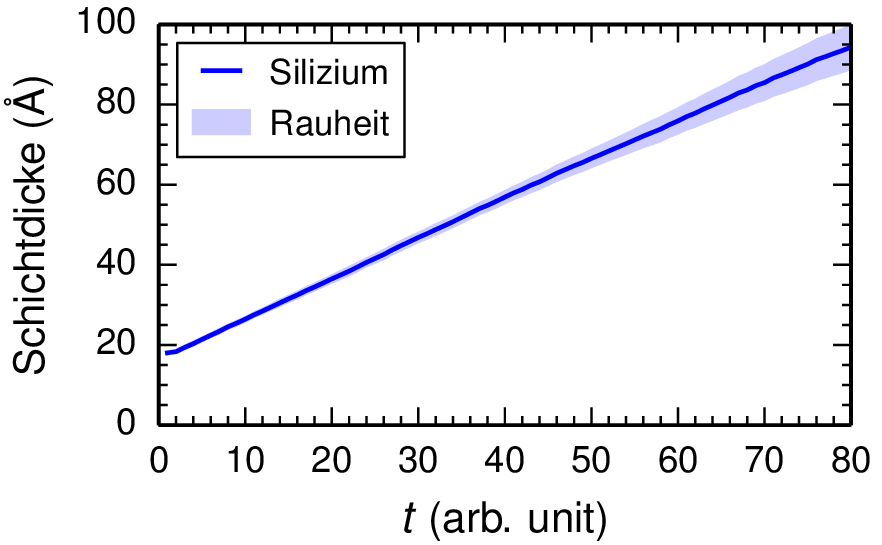
\includegraphics[width=\textwidth]{Si111_combined}
    \subcaption{Dicke und Rauheit der Schicht}
    \label{fig:siliconresults-a}
  \end{subfigure}
  \hfill
  \begin{subfigure}[t]{\subfigwidth}
    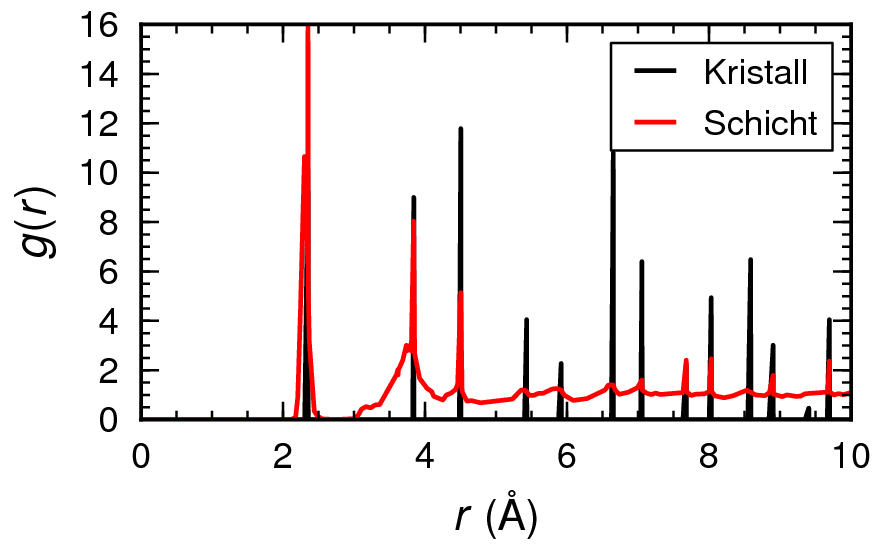
\includegraphics[width=\textwidth]{si111_rdf}
    \subcaption{Radiale Verteilungsfunktion bei $t=80$}
    \label{fig:siliconresults-b}
  \end{subfigure}
  \caption[Struktur einer Silizium-PVD-Schicht aus Parsivald]{
    Struktur einer Silizium-PVD-Schicht aus Parsivald (\SI{10x10}{\nano\meter})
  }
  \label{fig:siliconresults}
\end{figure}

Zur Charakterisierung der Kristalleigenschaften der abgeschiedenen Schicht wurde ihre radiale Verteilungsfunktion berechnet, die bereits nach \SI{4}{\angstrom}, keine langreichweitige Ordnung mehr zeigt, weshalb von einer amorphen Schicht auszugehen ist, wobei das kristalline Substrat in der RDF in Form von Spitzen an den Gitterabständen zu erkennen ist.
Die mittlere Koordinationszahl von \num{3.99} stimmt zudem gut mit der Anzahl an Bindungen für Silizium, die bei \num{4} liegt, überein.
Somit zeigt sich die ReaxFF-Formulierung erfolgreich in der Darstellung der strukturellen Eigenschaften von Silizium.

Die Unebenheiten der Oberfläche, welche Tiefen von \SI{30}{\angstrom} erreichen können, liegen hauptsächlich in der Form vieler Nanoporen vor, welche eine maximale Breite von wenigen Nanometern haben (Abbildung~\ref{fig:siliconprofile}).
Im Gegensatz zu den Vertiefungen während der Kupfer-PVD (Abschnitt~\ref{copperpvd}) werden diese nicht vollständig mit dem weiteren Wachstum der Schicht geschlossen, sodass die Ausbildung über längere Zeiträume ermöglicht wird.
Die Rauheit der Oberfläche erreicht gegen Ende der Simulation einen RMS-Wert von \SI{1.15}{\nano\meter}, welcher nur um einen Faktor von \num{10} oberhalb der Rauheiten der zuvor betrachteten kristallinen Schichten liegt.
Durch die begrenzte Simulationszeit ist keine Aussage über den weiteren Verlauf der Rauheit möglich, die womöglich in einen sublinearen Verlauf durch Schließung der Unebenheiten übergehen kann.
Es ist ein schwacher Einfluss der Poren auf die Schichtdicke (Abbildung~\ref{fig:siliconresults-a}) erkennbar, welche gegen Ende der Simulation trotz konstanter PVD-Rate sublinear steigt.
Somit wird die Schichtdicke unterschätzt, was sich auch in der Dichte der Struktur von \SI{2.597}{\gpcc} (Referenzen~\cite{remes_optical_1998,renner_density_1973}: \SIrange{2.20}{2.30}{\gpcc}) zeigt.

Zur Untersuchung des Einflusses von Unterrelaxierung wurde eine Abscheidung bei \SI{500}{\kelvin} simuliert(Abbildung~\ref{fig:siliconunderrelaxedprofile}), die realistischen Prozessbedingungen entspricht, aufgrund der kurzen Relaxationszeit aber nicht zur vollständigen Relaxation am Adsorptionsort führt.
Es zeigen sich höhere Rauheiten, feinere Nanoporen und steilere Hänge, die zu einer hohen Porösität der Schicht führen, weshalb zu erwarten ist, dass mit höheren Relaxierungszeiten eine verringerte Porenbildung beobachtet werden kann.


\begin{figure}[p]
  \centering
  \captionsetup[subfigure]{singlelinecheck=false}
  \begin{subfigure}[t]{8.5cm}
    \begin{overpic}[width=\textwidth]{si111_surface_profile}
      \put(-8,0){\includegraphics{1nmscale}}
    \end{overpic}
  \end{subfigure}
  \begin{subfigure}[t]{2.0cm}
    \def\svgwidth{\textwidth}
    \begin{overpic}[width=0.83cm]{greyhalfscale}
      \put(0,0){\input{img/si111_surface_profile_halfscale.pdf_tex}}
    \end{overpic}
  \end{subfigure}
  \caption[Oberflächenprofil einer Silizium-PVD-Schicht]{
    Oberflächenprofil einer auf Si-(111) per PVD abgeschiedenen Schicht
  }
  \label{fig:siliconprofile}
\end{figure}

\begin{figure}[p]
  \centering
  \captionsetup[subfigure]{singlelinecheck=false}
  \begin{subfigure}[t]{8.5cm}
    \begin{overpic}[width=\textwidth]{si111_underrelaxed_profile}
      \put(-8,0){\includegraphics{1nmscale}}
    \end{overpic}
  \end{subfigure}
  \begin{subfigure}[t]{2.0cm}
    \def\svgwidth{\textwidth}
    \begin{overpic}[width=0.79cm]{greyscale}
      \put(0,0){\input{img/si111_underrelaxed_profile_scale.pdf_tex}}
    \end{overpic}
  \end{subfigure}
  \caption[Oberflächenprofil einer unterrelaxierten Siliziumschicht]{
    Oberflächenprofil einer unterrelaxierten, porösen Silizium-PVD-Schicht
  }
  \label{fig:siliconunderrelaxedprofile}
\end{figure}
